\setcounter{part}{0}
\setcounter{chapter}{0}
\setcounter{section}{0}
\renewcommand{\thechapter}{\arabic{chapter}}
\renewcommand{\thepart}{\arabic{part}}
\renewcommand{\thesection}{\arabic{section}}

% appendix product backlog azure devops

\section{Product backlog Azure DevOps}

\begin{figure}[H]
    \centering
    \fbox{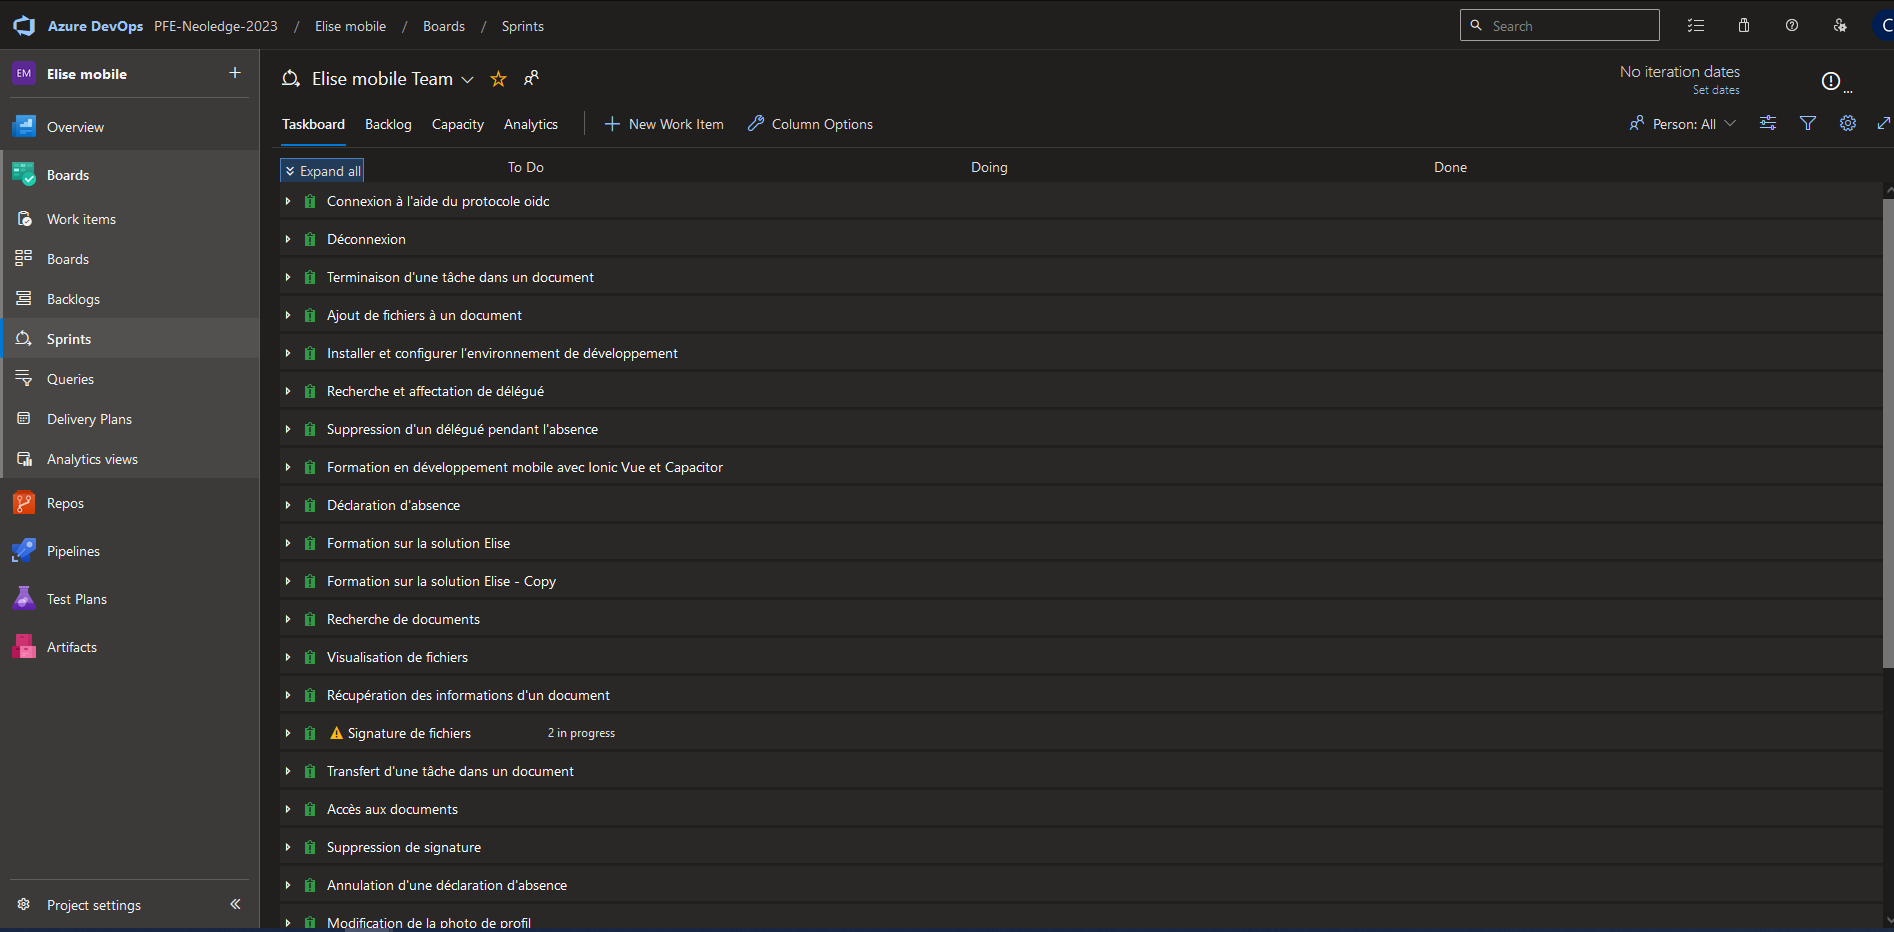
\includegraphics[width=0.8\textwidth]{capture_azure_devops}}
    \caption{Product backlog Azure DevOps}
    \label{fig:product_backlog_azure_devops}
\end{figure}

\label{appendix:product_backlog_azure_devops}



\section{neo-pdf-viewer}

\subsection{Fonctionnalité de l'affichage des images}

Pour prendre en charge les fichiers de type image dans notre package "neo-pdf-viewer", nous avons suivi les étapes suivantes :
\begin{itemize}
    \item \textbf{Ajouter un filtre de type de fichier :} Nous avons ajouté un filtre pour les fichiers de type image dans le composant "neo-pdf-viewer" pour mieux gérer les fichiers de différents types.
    \item \textbf{Ajouter un composant d'affichage d'image :} Nous avons utilisé le composant "img" de HTML pour afficher les images dans "neo-pdf-viewer".
\end{itemize}

L'ajout de la fonctionnalité d'affichage des images à "neo-pdf-viewer" nous a permis d'offrir une meilleure expérience utilisateur en affichant les images dans le même composant que les fichiers PDF.

\begin{figure}[H]
    \centering
    \fbox{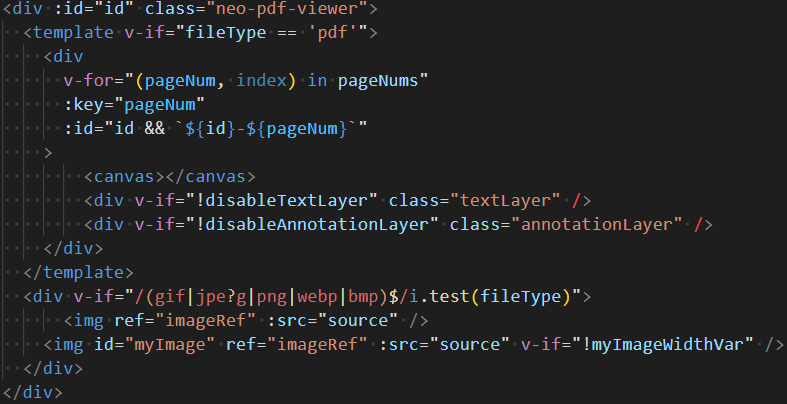
\includegraphics[width=0.8\textwidth]{code_image}}
    \caption{Code d'affichage des images}
    \label{fig:codedisplayimage}
\end{figure}

\subsection{Fonctionnalité de zoom}

Pour intégrer cette fonctionnalité de zoom dans notre package "neo-pdf-viewer", nous avons suivi les étapes suivantes :
\begin{itemize}
    \item \textbf{Évaluation des besoins :} Nous avons identifié le besoin de permettre aux utilisateurs de zoomer sur les documents PDF affichés dans "neo-pdf-viewer". Après avoir étudié différentes options, nous avons choisi d'utiliser la bibliothèque "vue3-pinch-scroll-zoom" pour sa facilité d'intégration et ses fonctionnalités complètes.
    \item \textbf{Configuration du composant :} Nous avons intégré la bibliothèque "vue3-pinch-scroll-zoom" pour englober chaque page de fichier dans un composant de zoom. 
    \item Mise a jour du package "neo-pdf-viewer" 
\end{itemize}

L'ajout de la bibliothèque "vue3-pinch-scroll-zoom" à "neo-pdf-viewer" nous a permis d'offrir une fonctionnalité de zoom fluide et intuitive

\begin{figure}[H]
    \centering
    \fbox{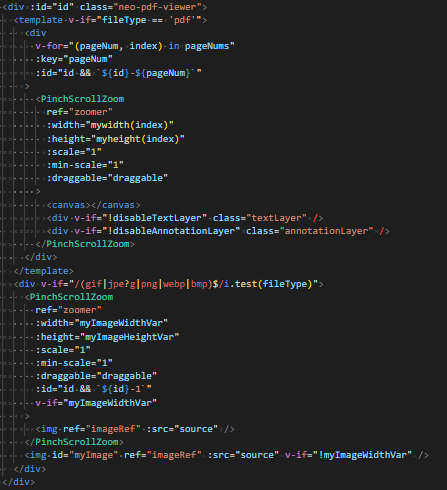
\includegraphics[width=0.7\textwidth]{capture_code_zoom}}
    \caption{Code de zoom}
    \label{fig:zoom_code}
\end{figure}

\label{appendix:neo-pdf-viewer}
